\chapter{Simulations}
\section{Plasma simulations}
\textbf{Why simulations}\\
Simulations because: Cheaper than experiments, more readily available to anyone, simulations allow us to study, understand and exploit these phenomena without the need to repeatedly perform expensive and intricate experiments...Furthermore, by having a simulated rather than physical experiment, one may avoid the uncertainties and noise present in the real world and may therefore investigate and even discover physical phenomena that are too sensitive to be detected in noisy data samples. To take advantage of simulations it is however crucial to know the accuracy by which the simulations model the physical situation and to understand the limitations that this imposes. For instance, as will be shown in section XXX, failing to model the experiment with high enough resolution can lead to phenomena emerging from purely numerical features in the simulations. One must therefore be confident that the results seen in simulations accurately represent the physics at hand, either by comparing the simulations to experimental data or theoretical calculations if available. The non-linear nature of the high-energy plasma wakefield phenomena that we wish to model in this project do not lend themselves easily to analytical treatments. To investigate these phenomena and provide useful results for future experiments we will make extensive use of simulations in this project.\\ 
Given that a plasma is no more than electrons and ions interacting electromagnetically, the response of such a plasma to the propagation of an electron bunch or laser pulse could in theory be simulated by solving Maxwell's equations for a set of initial conditions. This approach is however computationally intractable due to vast number, $>10^{15}$, of particles present in the simulations we need to perform. To circumvent this computational road block we make use of so-called Particle-In-Cell (PIC) codes, in which a large collections of physical microscopic particles are represented as smaller collections of macroscopic pseudo-particles on a grid. In this chapter we outline the general PIC approach and introduce the plasma physics PIC code EPOCH, which is used throughout this project. We further detail the modifications necessary to allow the hybrid beam dump scheme to be simulated on EPOCH. 

%In this chapter we introduce the plasma physics PIC code EPOCH, which is used throughout this project, and detail the modifications necessary to allow the hybrid beam dump scheme to be simulated. 

%The behaviour of these macro particles is then calculated and used as a representation of the response of the actual plasma.  where each macroscopic particle carries the total charge and mass of the microscopic particles it represents. 


\section{EPOCH}
%The simulations presented in this thesis are generated using the open-source plasma physics PIC simulation code \textsc{EPOCH},
The Extensible PIC Open Collaboration project (EPOCH) is an advance relativistic electromagnetic PIC code developed at the University of Warwick by XXX et al. [ref.user-manual]. EPOCH is now maintained and developed through the Collaborative Computational Project in Plasma Physics (CCP-Plasma), from which access to the code is granted to non-profit research laboratories and Universities [CCP website]. 
%Simulations  using EPOCH simply require users to specify the parameters and initial conditions of the simulations without the need to interact with the underlying PIC code.
The underlying code is written in Fortran and allows for simulations to be run on multiple parallel processors via MPI; this enables time-consuming simulations to be run on remote computing clusters. The core PIC code in EPOCH is based upon the field update and particle push algorithms of the Plasma Simulation Code (PSC) written by H. Ruhl []. This follows closely the standard PIC method outline in section \ref{sec:Particle-in-Cell Codes}. The main difference being in how the FTDT method is implemented and the inclusion of additional functionality to allow for more advanced features such as collisions, ionisation and quantum electrodynamic radiation to be simulated [epoch manual].  \\
\indent EPOCH is highly user-friendly; setting up simulations simply requires users to specify the parameters and initial conditions of the simulations without the need to interact with the underlying PIC code. Likewise, analysing and visualising data from a simulations is made easier through file-compatibility with Python, Matlab, IDL and VisIt, the details of which will be covered in this section.

\section{Particle-in-Cell Codes}
Particles are not on yee grid but fields are on yee grid. So rho and J need to be put on yee grid to find fields, and to find new particle positions the fields need to be calculated off-yee grid. However, since the electric field is sourced in part by magnetic flux variations, the fields are sovled at intermediate steps.\\
Since the fields are determined by the position and velocity of the particles, which in turn are determined by the fields, these can not be calculated simulataneously. In its simpelest form, PIC codes decouple these calculations by dividing each iterations step into four seperate parts.  
EM fields are fixed on grid, particles move freely
\label{sec:Particle-in-Cell Codes}
Starting from EM fields $\vec{E}_{(n)},\vec{B}_{(n)}$ and charge current $\vec{J}_{(n)}$ present at iteration $n$ [at a specific position, middle of Yee grid?] we obtained the fields at the next time step $n+1$ by computing the resulting fields and currents at an intermediate half-way step $n+1/2$. We do this by first computing the change in the electric field, using Ampere's law, $\Delta \vec{E}_{(n)}$ which we add to our current field such that
\begin{equation}
\vec{E}_{(n+1/2)}=\vec{E}_{(n)}+\frac{\Delta t}{2}\left(c^2\mathbf{\nabla}\times \vec{B}_{(n)}-\frac{\vec{J}_{(n)}}{\epsilon_0}\right)
\end{equation}
from this the magnetic field is given by
\begin{equation}
\vec{B}_{(n+1/2)}=\vec{B}_{(n)}-\frac{\Delta t}{2}\left(c^2\mathbf{\nabla}\times \vec{E}_{(n+1/2)}\right)
\end{equation}
(at which point the particle pusher, detailed below, updates the current to $\vec{J}_{(n+1)}$)\\
at which point we need to update the current to $\vec{J}_{(n+1)}$ in order to proceed finding the fields at time step $n+1$. This is done using the particle pusher. We update the position of each particle 
\begin{equation}
\vec{x}_{(n+1/2)}=\vec{x}_{(n)}+\frac{\Delta t}{2}\vec{v}_{(n)}
\end{equation}
from which we also obtain the intermediate velocity $\vec{v}_{(n)}$ [correct?]. Using the Lorentz force law we then compute the force $\vec{F}_{(n)}=\Delta p/\Delta t$ which gives the momentum at $n+1$ as
\begin{equation}
\vec{p}_{(n+1)}=\vec{p}_{(n)}+q\Delta t\left[\vec{E}_{(n+1/2)}\left(\vec{x}_{(n+1/2)}\right)+\vec{x}_{(n+1/2)}\times\vec{B}_{(n+1/2)}\left(\vec{x}_{(n+1/2)}\right) \right]
\end{equation}
where, the electric fields are extrapolated (?) to the intermediate point $n+1/2$. Then, using $\vec{p}=\gamma m \vec{v}$, we can find the velocity at $n+1$, from which we then have the current $\vec{J}_{(n+1)}$. We then reverse the order of computing such that the magnetic field is calculated prior to the electric field,
\begin{align}
&\vec{B}_{(n+1)}=\vec{B}_{(n+1/2)}-\frac{\Delta t}{2}\left(c^2\mathbf{\nabla}\times \vec{E}_{(n+1/2)}\right)\\
&\vec{E}_{(n+1)}=\vec{E}_{(n+1/2)}+\frac{\Delta t}{2}\left(c^2\mathbf{\nabla}\times \vec{B}_{(n+1)}-\frac{\vec{J}_{(n+1)}}{\epsilon_0}\right)
\end{align}
Using these fields when then calculate the new particles positions $\vec{x}_{(n)}$, we "push" the particles, thus completing the iteration step.
\begin{figure}
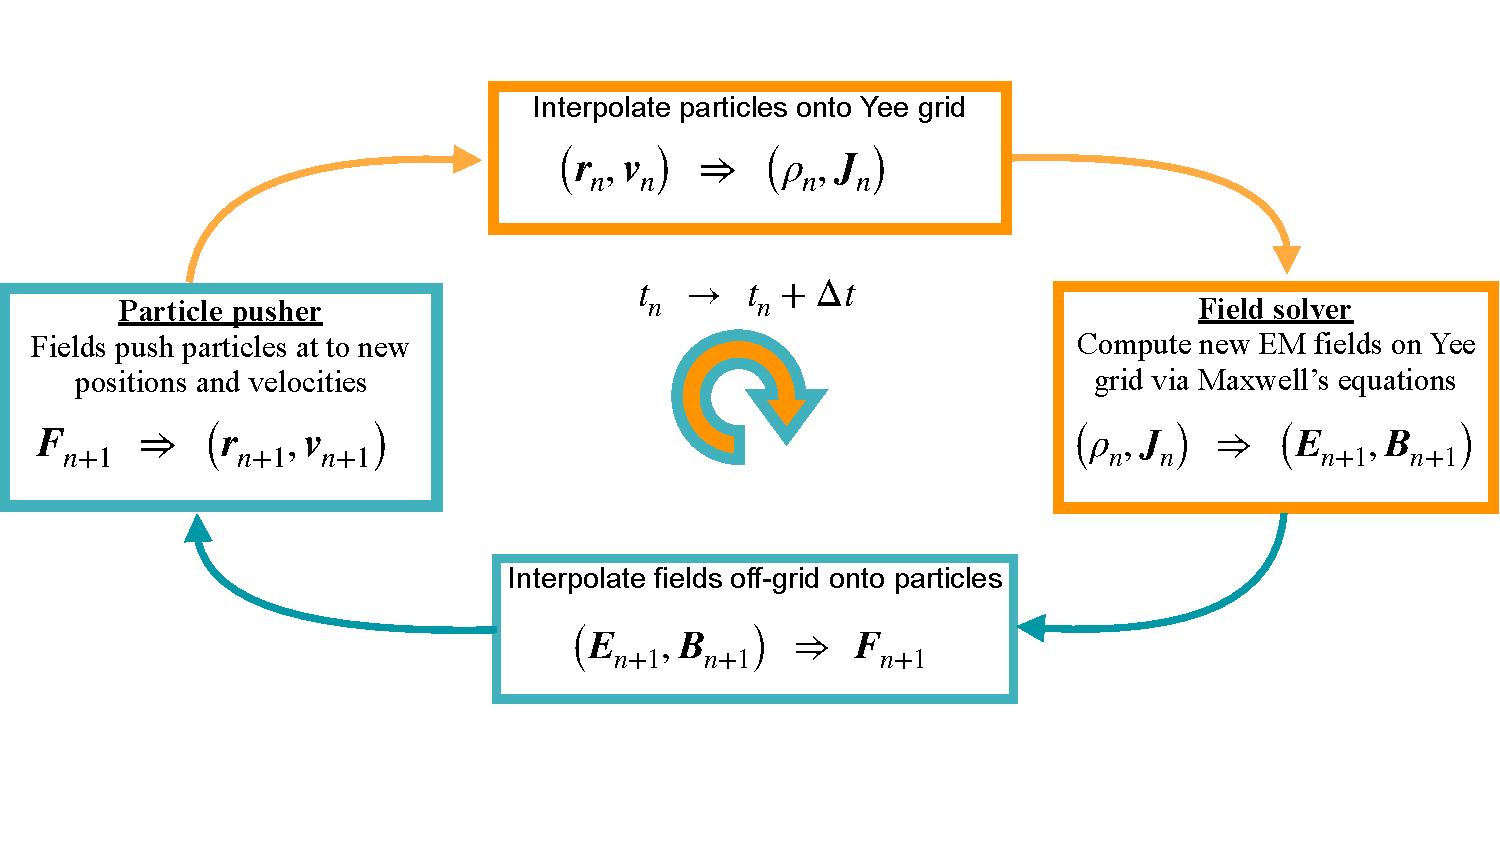
\includegraphics[width=\textwidth]{PIC_loop2.pdf}
\caption{The field update and particle push algorithm run b}
\end{figure}


\subsection{Input deck}
Once EPOCH has been downloaded and compiled the so-called input deck is essentially EPOCH's user interface. This is a file in which users specify the details of a simulations and it is this file that gets read by EPOCH and passed onto the core PIC algorithm. The input deck consists of blocks which define parameters for different features of the simulation. \\
\textbf{Explain control block first}, and what the restart does.
This specifies the grid that the simulations is to run on. We then populate this grid with plasma particles.
\textbf{Species block}, with explanation about analytical density distributions for plasma, and specify ppc.\\
The control and species blocks together define the resolution of the simulation. When setting up the resolution of the grid one has to make sure that the grid is sufficiently fine such that the smallest features of our physical system are resolved. This is to ensure that the simulation accurately models the physical system it is meant to represent, to the extent that missing small scale phenomena might alter the large scale outcome of the simulation. A finer grid however requires more macroparticles to fully populate the grid, which inevitably extents the computational time. In addition the time step $\Delta t$ aneeds to be suitably decreased as well. This is because of the so-called Courant-Friedrichs-Lewy (CFL) condition.  Any simulation introduces uncertainties in the final outcome due to the finite resolution. We need to make sure that the uncertainties introduces during each iteration do not build up and grow unbounded. \\

\subsection{Non-analytical bunch initialisation}
The hybrid scheme approach that the endeavour to investigate in this project relies on us being able to simulate a laser pulse propagating in front of a pre-saturated bunch. Previous investigations by our colleagues have shown that this is not a trivial task using the simulation software that have been tried. The issue with epoch in this regard is that everything that is to be included in the simulation need to be specified in the input deck and introduced at the beging of a simulation. Hence, simulations of the active beam dump are entirely possible in EPOCH, since a laser can be initialised in front of a bunch at $t=0$ and driven together. Introducing a laser at a later stage $t>0$ appeared however not to be possible. The majority of the work so far in this project has been concerned with solving this issue. The approach taken was to simulate the passive part first and then export the data of the saturated bunch into a new simulation which includes a laser driver. The structure of the SDF data files output by EPOCH are however not suitable for accessing and retrieving particular sets of data. A workaround was found by using VisIt to read the files and subsequently export only the data related to the electron beam. This data was subsequently read by EPOCH during the compilation stage in a specific file included in EPOCH. This file, usually left empty, allows users to over-ride section of the input file by assigning custom values to each of the macroparticles that are intialised in at the start of a simulation. Through this approach we are now able to define a simulation where a laser pulse is driven ahead of a standard bi-gaussian electron beam. By then over-riding the parameters for the electron beam we can then use the data from a pre-saturated bunch to reposition each macroparticle in the bi-gaussian to its corresponding position relative to the rest of the bunch. By also over-riding momentum parameters we can completely mould the bunch into the one we had exported after a passive beam dump. \\
\\
Real accelerators operate at a range of beam parameters tailored to specific reserach purposes. In order to avoid having to set up week-long simulations for each minor change of parameters it is crucial to understand the theory underlying these plasma wakefield phenomena and to see to what extent the theoretical predictions match the simulations

For any pracitactal implementation of the hybrid scheme to an existing experiment it 
